\documentclass{article}
\usepackage{graphicx, amsmath, float, siunitx, hyperref, mathtools} % Required for inserting images
\usepackage[ngerman]{babel}
\usepackage{biblatex, csquotes}
\addbibresource{refs.bib}
\usepackage[
  locale=DE,
  separate-uncertainty=true,
  per-mode=symbol
]{siunitx}

\sisetup{output-decimal-marker = {,}}

\DeclareSIUnit\gauss{G}

\newcommand{\abb}{{\color{red}\textbf{{ABB.XYZ}}} }
\newcommand{\Oszi}{Oszilloskop }

\usepackage{caption}
\usepackage{subcaption}

\usepackage{csvsimple}
\usepackage{comment}
\usepackage{booktabs}

\title{Praktikum V - Kern- und Teilchenphysik\\Versuch 518 - Höhenstrahlung}

\author{Tom Chelius und Alican Özcagi}
\date{07. Mai 2025}


\begin{document}
\maketitle
\newpage
\tableofcontents

\newpage

\section{Einleitung}
Die Höhenstrahlung ist eine Form von ionisierender Strahlung, die in der Erdatmosphäre vorkommt. 
Sie besteht hauptsächlich aus hochenergetischen Teilchen, die aus dem Weltraum auf die Erde treffen. 
Diese Teilchen können Protonen, Elektronen und Atomkerne sein, die mit sehr hohen Geschwindigkeiten reisen. 
Die Höhenstrahlung entsteht durch verschiedene astrophysikalische Prozesse, wie z.B. Supernova-Explosionen oder 
die Wechselwirkung von kosmischer Strahlung mit der Erdatmosphäre.
In diesem Versuch werden wir die Höhenstrahlung auf seine Winkelverteilung untersuchen.
Außerdem werden wir die Lebensdauer der kosmischen Myonen bestimmen.

\section{Theorie}
Um diesen Versuch verstehen zu können, ist es wichtig, die Grundlagen der Höhenstrahlung und der Teilchhen zu kennen, sowie die 
Messinstrumente die wir verwenden werden. 

\subsection{Kosmische Strahlung}
Die kosmische Strahlung besteht aus hochenergetischen Teilchen, die aus verschiedenen Quellen stammen.
Sie kann hauptsächlich in 3 Kategorien unterteilt werden:
\begin{itemize}
    \item Teilchen die aus der Sonne stammen (Sonnenstrahlung) $\approx$ bis $\SI{10}{\giga\electronvolt}$
    \item Teilchen die aus dem interstellaren Raum stammen (Galaktische Strahlung) $\approx$ ab $\SI{1}{\giga\electronvolt}$ 
    \item Teilchen die aus dem intergalaktischen Raum stammen (Extragalaktische Strahlung)  $\approx$ bis $\SI{10}{\exa\electronvolt}$
\end{itemize}
Die Teilchen die auf die Erdatmosphäre treffen, sind hauptsächlich Elektronen, Photonen, Protonen und vollständig 
ioniersierte Kerne. Je nach Quelle sind die Energien der Teilchen unterschiedlich.
Die kosmische Strahlung wird in primäre und sekundäre Strahlung unterteilt.
Die primäre Strahlung sind die Teilchen die direkt aus dem Weltraum auf die Erde treffen.
Die sekundäre Strahlung sind die Teilchen die durch die Wechselwirkung der primären Strahlung mit der Erdatmosphäre entstehen.
Diese Entstehung der sekundären Strahlungen wird als Teilchenschauer bezeichnet, weil aus einem primären Teilchen viele sekundäre Teilchen entstehen. 
Sie wird aus den folgenden Prozessen gebildet:
\begin{itemize}
    \item \textbf{Kernreaktion:} Die Primäre Strahlung trifft auf die Atomkerne der Erdatmosphäre und erzeugt Sekundäre Teilchen.
    \item \textbf{Teilchenschauer:} Die Sekundären Teilchen erzeugen weitere Sekundäre Teilchen, die sich in alle Richtungen ausbreiten.
    \item \textbf{Ionisation:} Die Sekundären Teilchen ionisieren die Luftmoleküle und erzeugen weitere Elektronen.
\end{itemize}
Diese Teilchenschauer bestehten aus 3 Bereichen, wie in der Abbildung \ref{fig:Teilchenschauer} dargestellt.
\begin{figure}[H]
    \centering
    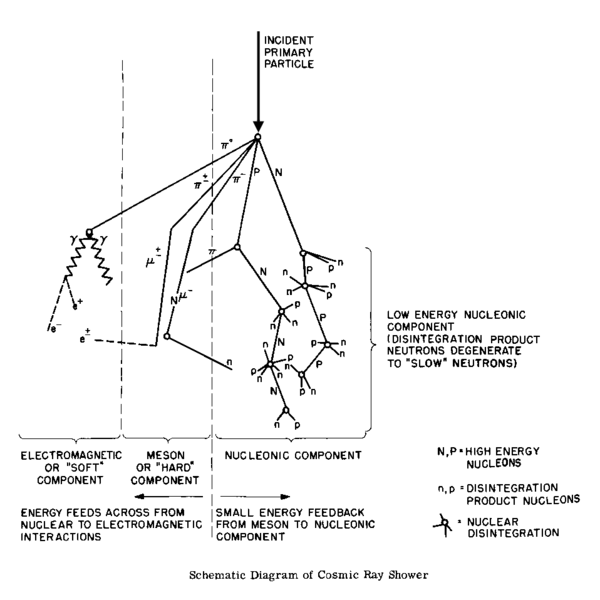
\includegraphics[width=0.5\textwidth]{figures/Teilchenschauer.png}
    \caption{Schematische Darstellung eines Teilchenschauers \cite{shower}}
    \label{fig:Teilchenschauer}
\end{figure}
\begin{itemize}
    \item Elektomagnetische-Komponente: Diese besteht aus Photonen und Elektronen und wird die \enquote{Softe} Komponente genannt.
    \item Mesonen-Komponente: Diese besteht aus Myonen und wird die \enquote{Harte} Komponente genannt.
    \item Nukleonen-Komponente: Diese besteht aus Protonen und Neutronen.
\end{itemize}
Die Teilchen die wir auf der Erdatmosphäre messen, sind hauptsächlich Myonen, da diese die Teilchen sind die mit am weitesten
in die Erdatmosphäre eindringen können und noch in hohen Quantitäten vorhanden sind.
In der Abbildung \ref{fig:Fluss} ist der vertikale Fluss zur atmosphärischen Eindringtiefe und zur Höhe der Erdoberfläche dargestellt.
\begin{figure}[H]
    \centering
    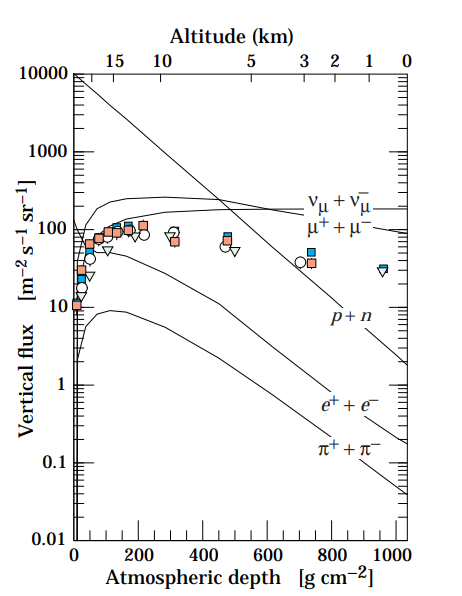
\includegraphics[width=0.5\textwidth]{figures/Fluss.png}
    \caption{Vertikaler Fluss zur atmosphärischen Eindringtiefe \cite{Naka}}
    \label{fig:Fluss}
\end{figure} 

\subsection{Energieverlust von Teilchen in Materie}
Durch die Wechselwirkung der Teilchen mit der Materie verlieren sie Energie. Der mittlere Energieverlust eines Teilchens in Materie wird durch die Bethe-Bloch-Gleichung (\cite{Bethe}) beschrieben.
\begin{equation*}
    -\frac{\mathrm{d}E}{\mathrm{d}x} = \frac{4\pi n z^2}{m_e c^2} \cdot \frac{e^4}{(4\pi \varepsilon_0)^2} \cdot \frac{1}{\beta^2} \cdot \left[ \ln\left(\frac{2 m_e c^2 \beta^2 }{I\cdot (1-\beta^2)}\right) - \beta^2 \right]    
\end{equation*}
Dabei ist $E$ die Energie des Teilchens, $x$ die Wegstrecke in der Materie, $m_e$ die Masse des Elektrons, $c$ die Lichtgeschwindigkeit, $Z$ die Ordnungszahl des Materials, $A$ die Massenzahl des Materials, $e$ die Elementarladung, $\varepsilon_0$ die elektrische Feldkonstante, $\beta = \frac{v}{c}$ die Geschwindigkeit des Teilchens relativ zur Lichtgeschwindigkeit und $I$ die Ionisationsenergie des Materials. 

Die Bethe-Bloch-Gleichung zeigt, dass der Energieverlust von der Geschwindigkeit des Teilchens, der Ordnungszahl des Materials und der Ionisationsenergie des Materials abhängt.
Da aber der Energieverlust von Teilchen in Materie ein statistischer Prozess ist, wird seine Verteilung durch die Landau-Verteilung (\cite{Landau}) beschrieben.
\begin{equation*}
    f(x) = \frac{1}{\sqrt{2\pi}} \cdot e^{-\frac{1}{2} \left(\frac{x - \mu}{\sigma}\right)^2}    
\end{equation*}
Dabei ist $\mu$ der Mittelwert und $\sigma$ die Standardabweichung der Verteilung.
Wie in der Abbildung \ref{fig:Landau} zu erkennen ist der Verlauf der Landau-Verteilung nicht symmetrisch, sondern hat einen langen Schwanz in Richtung höherer Energieverluste.
\begin{figure}[H]
    \centering
    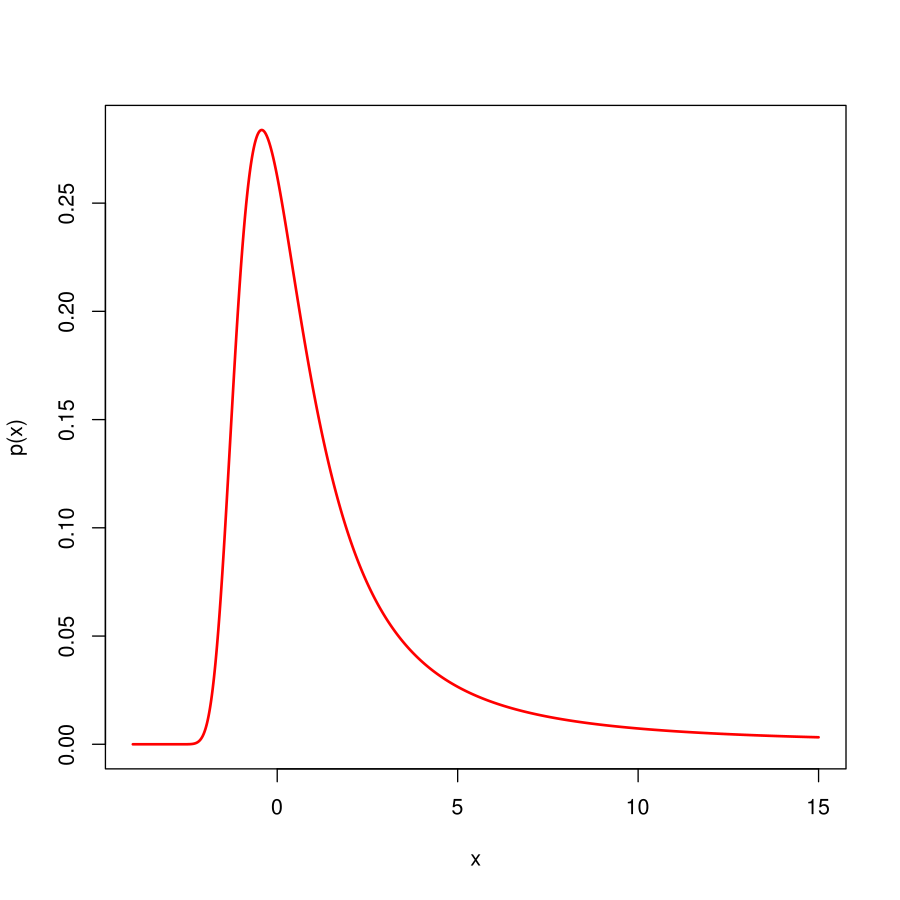
\includegraphics[width=0.5\textwidth]{figures/Landau.png}
    \caption{Landau-Verteilung \cite{Landau}}
    \label{fig:Landau}
\end{figure}

\subsection{Standardmodell}
Das Standardmodell der Teilchenphysik ist eine Theorie, die die fundamentalen Teilchen und ihre Wechselwirkungen beschreibt.
Aus diesem können die Eigenschaften der Teilchen abgeleitet werden. Das Standardmodell ist in der Abbildung \ref{fig:Standardmodell} dargestellt.
\begin{figure}[H]
    \centering
    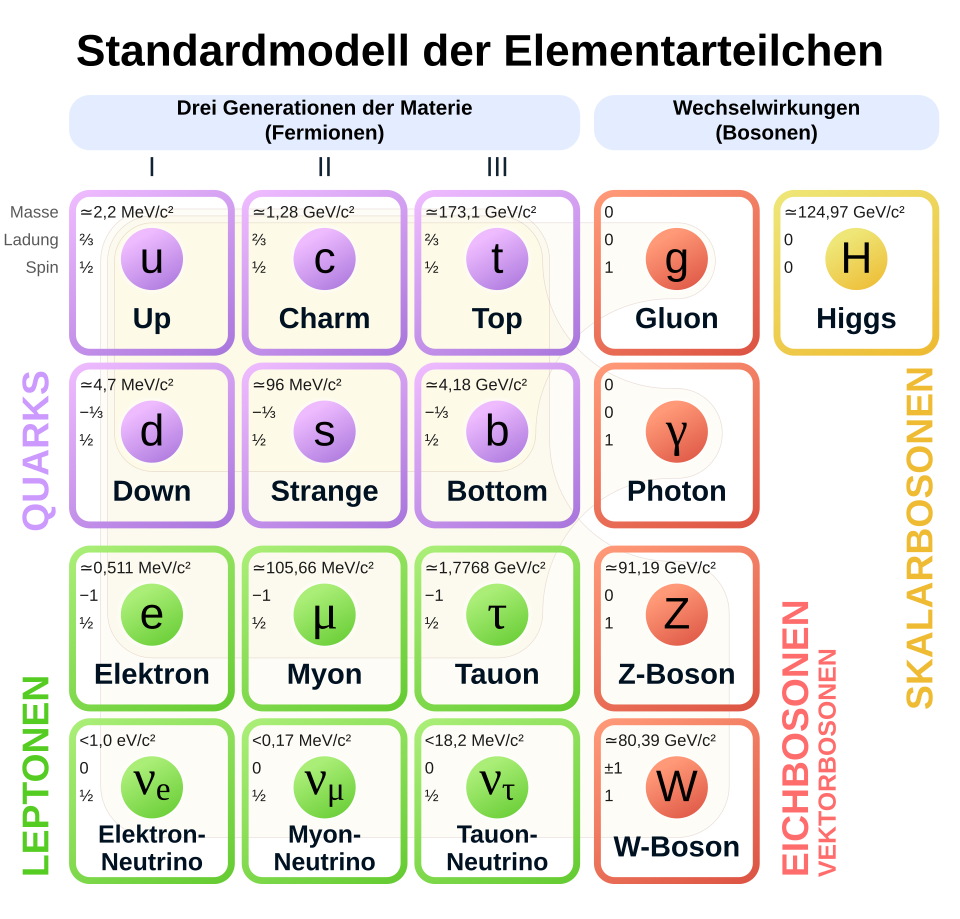
\includegraphics[width=0.5\textwidth]{figures/Standardmodell.png}
    \caption{Das Standardmodell der Teilchenphysik \cite{Standardmodell}}
    \label{fig:Standardmodell} 
\end{figure}
\textbf{\color{red}MEHR SCHREIBEN ODER RAUSNEHMEN}

\subsection{Szintillator und Photomultiplier}
Szintillationsdetektoren basieren auf ausgesendeten Lichtteilchen (Photonen). Ionisierende Strahlung trifft auf das szintillierende Material 
und erzeugt durch Ionisation eine Kaskade an Elektron-Loch-Paaren. Dies geschieht durch Prozesse, wie im Abschnitt \enquote{Materie und Photonen Wechselwirkung} 
beschrieben. Die herausgelösten Elektronen überwinden somit die Bandlücke und landen im Leitungsband. Dort sind sie (sowie ihre hinerlassenen Löcher) 
als frei bewegliche Ladungen delokalisiert und können an anderer Stelle auf aktive Zentren stoßen. Diese aktiven Zentren kommen von der Dotierung mit 
einem anderen Material (hier Thallium) in unser Gitter. An diesen aktiven Zentren können sich die Elektron-Lochpaare über ein anderes Energieniveau 
lumineszierend abbauen, wobei Photonen im nahen bis sichtbaren Bereich ausgesendet werden. Wir verwenden in dem Versuch einen 
Natrium-Iod-Szintillationsdetektor den wir kurz NaI-Detektor nennen.

Der beschriebene Prozess ist auch nochmal in der Abbildung \ref{fig:SzintillatorBandlücke} dargestellt.

\begin{figure}
    \centering
    \includegraphics[width=1\linewidth]{figures/Szintillator_Bändermodell.png}
    \caption{Darstellung des Bändermodell eines Szintillators \cite{Wer}}
    \label{fig:SzintillatorBandlücke}
\end{figure}

In dem Photomultiplier lösen die Photonen dann Elektronen aus der Photokathode. Eine Verstärkung wird über ein Dynodensystem realisiert. Hierbei gilt eine Dynode als Kathode, während die nächste als Anode wirkt und zwischen jedem Dynodenpaar wird das Signal verstärkt. Veranschaulicht wird der Effekt in der Abbildung \ref{fig:AufbauSzinti}. Der Photomultiplier ist an eine Hochspannungsquelle angeschlossen und die Dynoden haben über eine Reihe an Spannungsteilern zu immer höhere elektrische Potentiale.

\begin{figure}[H]
    \centering
    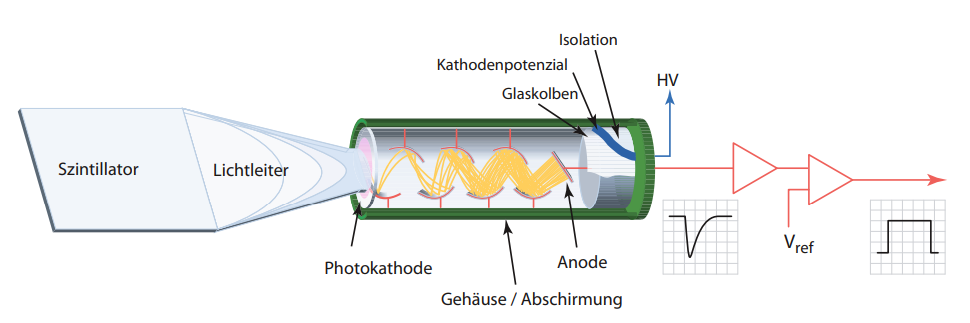
\includegraphics[width=1\linewidth]{figures/SzintillatorAufbau.png}
    \caption{Aufbau eines Szintillator \cite{Wer}}
    \label{fig:AufbauSzinti}
\end{figure}

\subsection{Logische Schaltung: Diskriminator, Koinzidenz-Module und FPGA}
Um aus den gemessenen Analogen Signalen digitale Signale zu erzeugen, verwenden wir einen Diskriminator. 
Dieser trennt die Signale in zwei Bereiche: Ein Signal unterhalb der Schwelle wird als \enquote{0} und ein Signal oberhalb der Schwelle als \enquote{1} gewertet. 
Hiermit können wir Rauscheffekte vermeiden und zusätzlich gibt der Diskriminator uns die Möglichkeit, die Signaldauer einzustellen.

Das Koinzidenz-Modul wirkt als ein logisches Und, es nimmt eine Menge an Signalen entgegen und gibt nur dann ein Signal aus, 
wenn alle Signale gleichzeitig anliegen. Das Koinzidenz-Modul wird verwendet damit einem durchfliegenden Teilchen ein Winkel zugeordnet werden kann, 
dazu wird geschaut, ob das Signal durch meherere Szintillatoren in einer Reihe gleichzeitig ausgelöst wird.

Ein FPGA (Field Programmable Gate Array) ist ein programmierbarer Logikbaustein und wird in diesem Versuch verwenden um Programme zu erstellen, die die Winkelverteilung
und die Lebensdauer der Myonen bestimmen können.
Die Programmierung wird in der LABView-Umgebung durchgeführt.
\subsection{Zufallskoinzidenz} 
Die Zufallskoinzidenz ist ein Effekt, der auftritt, wenn zwei oder mehr Ereignisse zufällig gleichzeitig auftreten. 
Dies ist relevant, weil wir bei der Bestimmung der Winkelverteilung und der Lebensdauer der Myonen wissen müssen, wie oft die Signale durch mehr als ein Teilchen
ausgelöst werden. Hierzu bestimmen wir die Zufallskoinzidenzrate um die Rate der echten Koinzidenzen zu bestimmen.
Diese kann auf 2 Arten bestimmt werden:
\begin{itemize}
    \item \textbf{zeitliche Zufallskoinzidenzrate:} Hierbei wird die Zeit der 3 Detektoren zeitlich so verschoben, dass ein einzelnes Teilchen keine Koinzidenz erzeugen kann.
        Es müssen also 3 Teilchen durch die 3 Detektoren fliegen um eine Koinzidenz zu erzeugen.
    \item \textbf{räumliche Zufallskoinzidenzrate:} Hierbei wird die räumliche Anordnung der Detektoren so gewählt, dass ein einzelnes Teilchen keine Koinzidenz erzeugen kann.
        Dabei müssen mindestens 2 Teilchen durch 2 Detektoren fliegen um eine Koinzidenz zu erzeugen.
\end{itemize}   

\section{Druchführung}
Dieser Versuch besteht aus 2 Teilen. Im ersten Teil soll die Winkelverteilung der Höhenstrahlung bestimmt werden und im zweiten Teil die Lebensdauer der Myonen.

\subsection{Winkelverteilung}
Um die Winkelverteilung der Höhenstrahlung zu bestimmen, werden 24 Szintillatoren verwendet, die in einem Kreis angeordnet sind, ein 25. Szintillator ist in der Mitte des Kreises angebracht.
Der Kreis hat einen Durchmesser von 1,5 m.
Je zwei gegenüberliegende Szintillatoren und der mittlere (Z25) sind mit einem Koinzidenzmodul verbunden, das die Signale der drei Szintillatoren verarbeitet, somit kann der Raum in 12 Sektoren unterteilt werden, 
welche je einen Raumwinkel von $\SI{15}{\degree}$ abdecken.
Alle Szintillatoren sind mit einem Diskriminator verbunden, der die Signale in digitale Signale umwandelt.
Dieser Aufbau ist in der Abbildung \ref{fig:AufbauWinkelverteilung} dargestellt.
\begin{figure}[H]
    \centering
    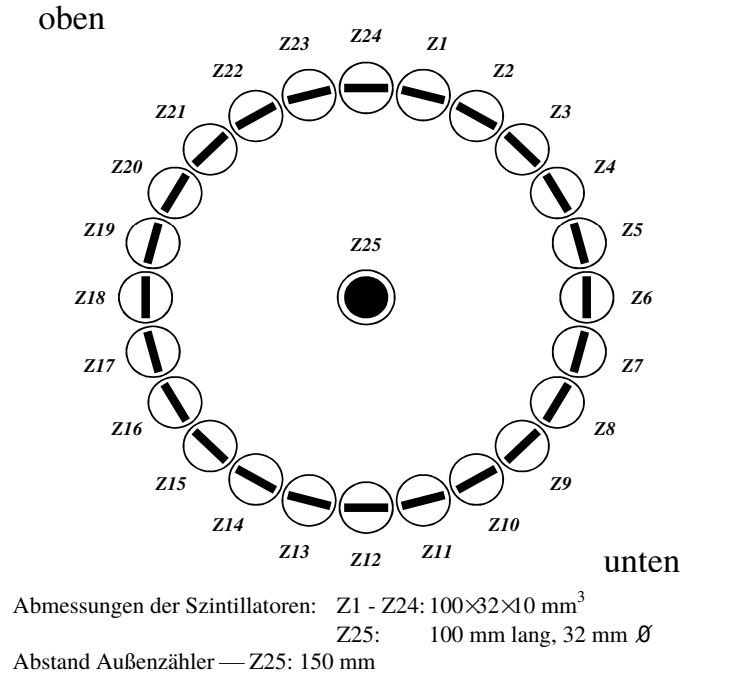
\includegraphics[width=0.7\textwidth]{figures/Aufbau_Winkelverteilung.png}
    \caption{Aufbau der Winkelverteilungsmessung\cite{Anleitung}}
    \label{fig:AufbauWinkelverteilung}
\end{figure}


\subsubsection*{Schwellenspannung D12}
Damit die Szintillatoren und der Photomultiplier richtig arbeiten, muss die Schwellenspannung eingestellt werden.
Hierzu wurde mit Hilfe von LABView ein Programm geschrieben, dass die Schwellenspannungen von $\SI{-50}{\milli\volt}$ bis $\SI{-200}{\milli\volt}$ variiert und die Anzahl an Koinzidenzen misst.

Das Programm ist im Anhang zu finden \ref{fig:LABView1} bis \ref{fig:LABView4}.
In diesem Programm wird zunächst die NIM-Box eingelesen. Anschließend werden die Diskriminatoren der Szinitillatoren D1, D2, D23, D24, D25 und D12 initialisiert, sodass das FPGA diese erkennen kann.	
Die Schwellenspannungen der Diskriminatoren D1, D2, D23 und D24 sind bereits vorgegeben.
Nun werden folgende Signale gezählt:
\begin{itemize}
    \item \textbf{Z25}
    \item \textbf{Z12}
    \item ODER Signal von \textbf{D24}, \textbf{D23}, \textbf{D1} und \textbf{D2} gebildet	
    \item Koinzidenzsignal von \textbf{D12} und \textbf{ODER Signal}  	
\end{itemize}
Dann wird in einer Schleife die Schwellenspannung von D12 von $\SI{-50}{\milli\volt}$ bis $\SI{-200}{\milli\volt}$ in Schritten von $\SI{-10}{\milli\volt}$ variiert.
Im letzten Schritt werden die gemessenen Zählwerte in ein Array geschrieben und in eine Txt-Datei gespeichert.
Hieraus kann dann die geeinete Schwellenspannung abgeleitet werden und
damit kann dann eine vom Höhenstrahlungsfluss unabhängig Analyse von der Schwellenspannung durchgeführt werden.

\subsubsection*{Langzeitmessung}
Wenn die Schwellenspannung eingestellt ist, wird eine Langzeitmessung durchgeführt.
Hierzu wurde ein Programm zur Winkelverteilungsmessung vorgegeben. Dieser funktioniert nach dem Prinzip der Koinzidenzmessung, der genaue Aufbau ist in der Abbildung \ref{fig:AufbauWinkelverteilungLangzeit} schmematisch dargestellt.
\begin{figure}[H]
    \centering
    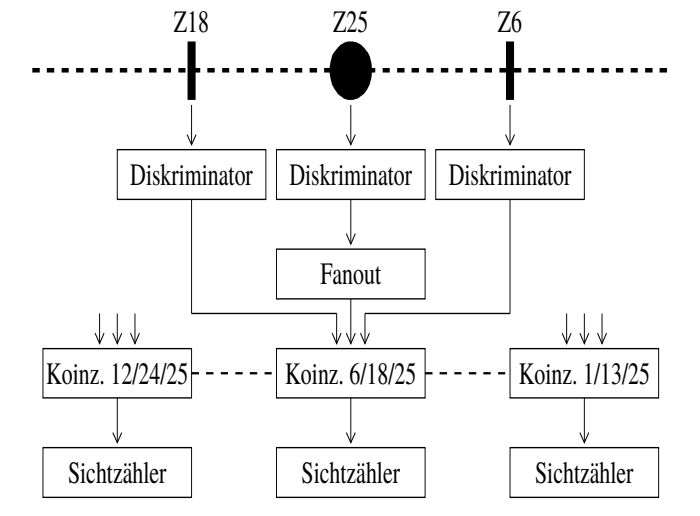
\includegraphics[width=1\textwidth]{figures/SchematischWinkelverteilung.png}
    \caption{Schematischer Aufbau der Winkelverteilungsmessung}
    \label{fig:AufbauWinkelverteilungLangzeit}
\end{figure}
Es werden je 2 Detektoren die sich gegenüberliegende Detektoren mit der mittleren Szintillatoren Z25 durch Diskriminatoren in ein Kooinzidenzmodul geschickt und dort von einem Stichzähler gezählt.
Diese Messung wurde mit einer Dauer von $\SI{598215}{\second}$ durchgeführt, dies entspricht etwa einer Woche.


\subsection{Lebensdauer}
Auch bei der Lebensdauermessung der Myonen müssen erst die Schwellenspannungen der Diskriminatoren eingestellt werden.
Dabei wurde ein anderes Verfahren verwendet, als bei der Winkelverteilungsmessung.
Bei dieser Methode wurde jeder Szintillator an 2 Diskriminatoren angeschlossen, diese Bilden den Messkreis (in Abbildung \ref{fig:AufbauLebensdauer} dunkel Blau) und den Monitorkreis (in Abbildung \ref{fig:AufbauLebensdauer} Rot).
\begin{figure}[H]
    \centering
    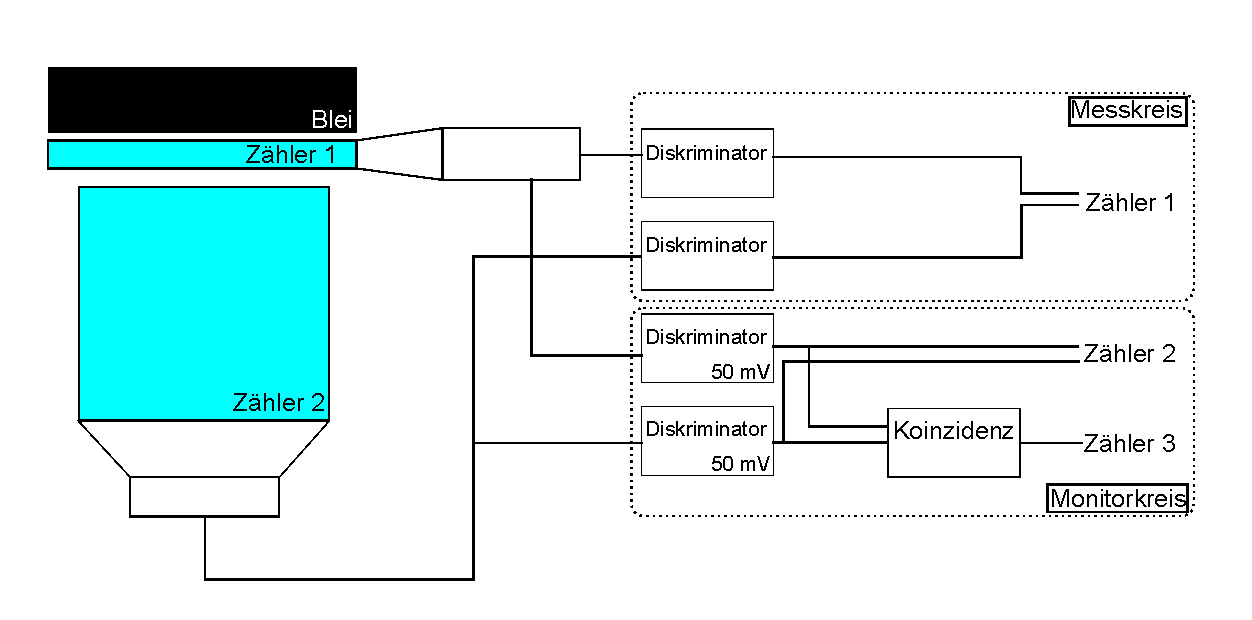
\includegraphics[width=1\textwidth]{figures/Aufbau_Lebensdauermessung.pdf}
    \caption{Schmatischer Aufbau für die Bestimmung der Schwellenspannung für die Lebensdauermessung}
    \label{fig:AufbauLebensdauer}
\end{figure}
Dann wurde im Messkreis die Schwellenspannung des einen Szintillators variiert, während die Schwellenspannung des anderen Szintillators konstant gehalten wurde.
Die Schwellenspannungen im Monitorkreis wurden auf $\SI{-50}{\milli\volt}$ eingestellt und festgehalten.
Es wurde mit der variierten Schwellenspannung im Messkreis des einen Szintillators, die Anzahl an Ereignissen gezählt.
Damit kann dann die Schwellenspannung des Szintillators über den Monitorkreis normiert werden. 
Da während unserer Durchführung der dicke Szintillator defekt war konnten wir nur die Zählrate des dünnen Szintillators messen.
Daher konnten wir auch nicht die Messung zur Lebensdauer der Myonen durchführen. Die Daten zur Auswertung erhielten wir von den Tutoren.
Nachdem die Schwellenspannungen eingestellt wurden, kann mit der Schaltung aus der Abbildung \ref{fig:AufbauZerfall} die Lebensdauer der Myonen bestimmt werden.
\begin{figure}[H]
    \centering
    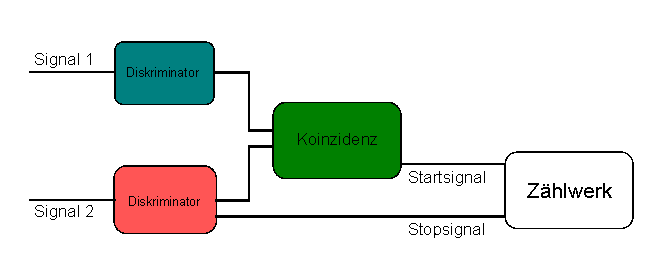
\includegraphics[width=1\textwidth]{figures/Aufbau_Zerfallsmessung.pdf}
    \caption{Aufbau der Lebensdauermessung mit Start- und Stop-Signal}
    \label{fig:AufbauZerfall} 
\end{figure}
Hierzu wird ein Start Signal ausgelöst, wenn ein Myon durch beide Szintillatoren fliegt und somit das Koinzidenzmodul auslöst. 
Wenn dies geschehen ist wird durch ein Schalt-Flip-Flop ein Gate geöffnet. Durch dieses Gate gelangt eine $\SI{20}{\mega\hertz}$-Pulsfrequenz auf zahn kaskadierte 1:20-Untersetzer mit
zugeordneten Sichtzählern. Nun kann es zu zwei Szenarien kommen, Ein Myon fliegt durch den Szintillator und löst das Koinzidenzmodul aus. Das Gate öffnet sich und die Zählrate wird gezählt, wenn:
\begin{itemize}
    \item ein Stop Signal innerhalb von $\SI{10}{\micro\second}$ ausgelöst wird, wird das Gate geschlossen und der Sichtzähler bleibt bei der Kodierung stehen. In dieser Zeit wird eine Totzeit-Generator gestartet
    und es kann für eine gewisse Zeit kein weiteres Start-Signal ausgelöst werden. Wenn die Totzeit abgelaufen ist, wird ein Reset-Impuls erzeugt und der Untersetzer auf Null zurückgesetzt.
    \item kein Stop-Signal innerhalb der $\SI{10}{\micro\second}$ erscheint, wird am Ende des Zählers ein Overflow-Impuls gesetzt, dieser lößt direkt ein Reset-Impuls aus, der den Zähler auf Null zurückgesetzt. 
\end{itemize}
Damit das Stop-Signal nicht durch Zufallskoinzidenzen sofort ausgelöst wird, wird das Start-Signal zeitverzögert.

\section{Auswertung}

\subsection{Winkelverteilung}
\subsubsection*{Schwellenspannung D12}
Aus der Messung der Schwellenspannung D12 (\ref{tab:SchwellenspannungWinkelverteilung}) ergibt sich eine geeignete Schwellenspannung von $\SI{-70}{\milli\volt}$.
Dieser wurde ermittelt, indem der erste Sattelwert aus der Auftragung von $N_\text{koin}/N_{25}$ gegen die Schwellenspannungen betrachtet wurde, 
dies ist zu sehen in der Abbildung \ref{fig:SchwellenspannungWinkelverteilung}.
\begin{figure}[H]
    \centering
    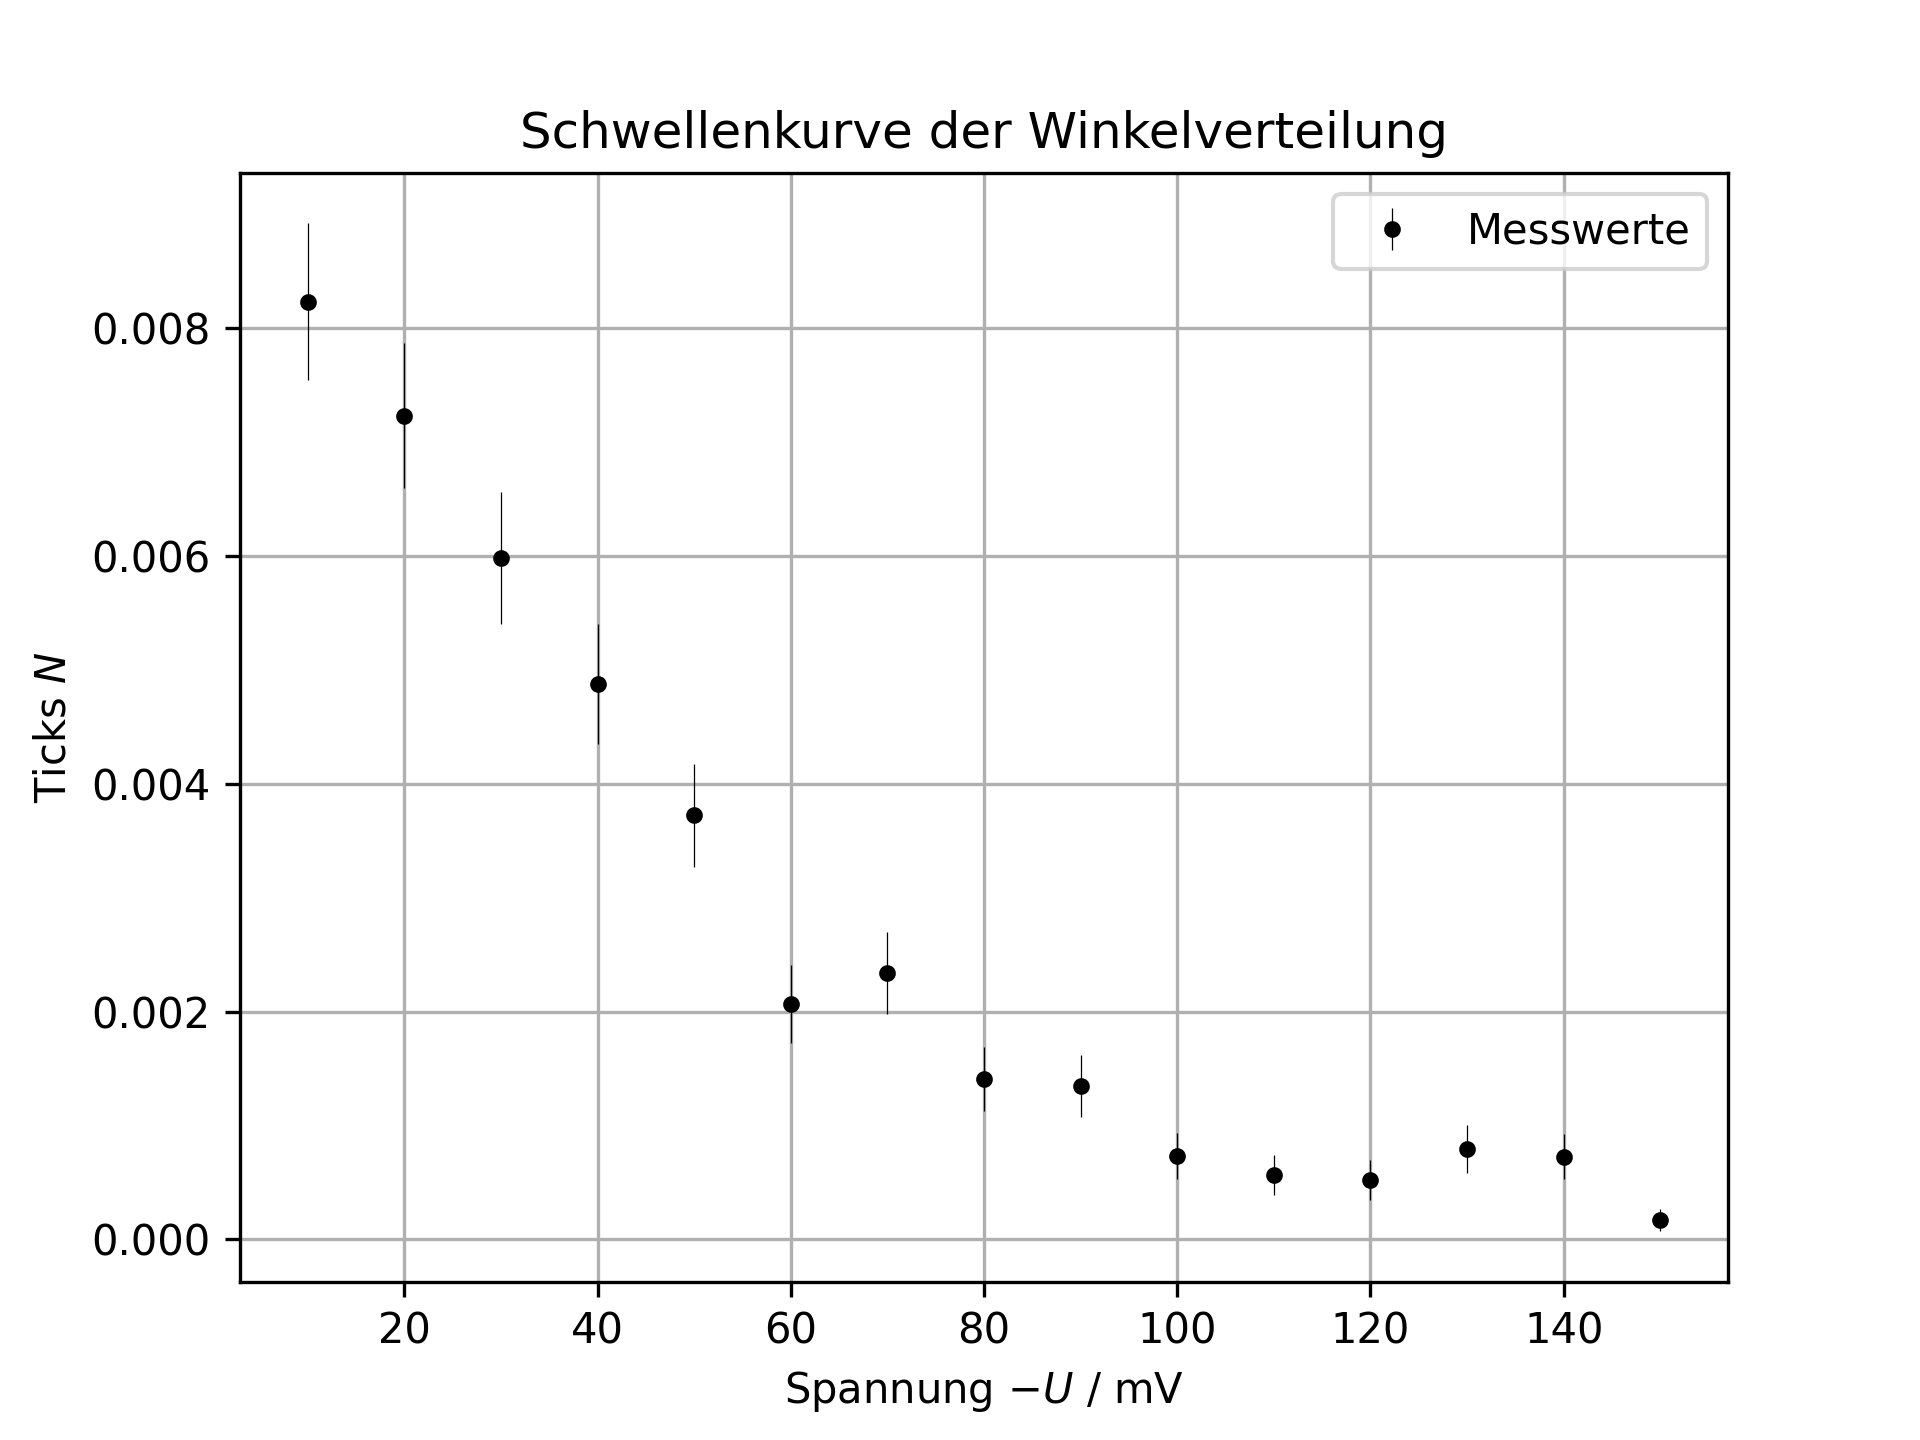
\includegraphics[width=1\textwidth]{figures/Schwellenspannung_Winkelverteilung.png}
    \caption{Auftragung zur Bestimmung der Schwellenspannung des Szintillators D12}
    \label{fig:SchwellenspannungWinkelverteilung}
\end{figure}
\subsubsection*{Anpassung der Winkelverteilung}
Nachdem die Schwellenspannung bestimmt und eingestellt wurde, wurde die Langzeitmessung druchgeführt, die gemessenen Werte sind im Anhang in der Tabelle \ref{tab:Winkelverteilung} hinterlegt.
An diese Werte wurde eine Cosinus und eine Gaussanpassung durchgeführt, diese sind in den Abbildungen \ref{fig:WinkelverteilungCosinus} und \ref{fig:WinkelverteilungGauss} dargestellt.
Bei den Anpassungen wurden die Rot markierten Werte nicht berücksichtigt, da diese offensichtlich ausreißer sind, wie diese Zustande kommen wird nachher im Abschnitt \enquote{Pulshöhenspektrum} genauer erklärt.
Die Anpassungsfunktionen sind zu sehen in der Gleichung \ref{eq:CosinusAnpassung} und \ref{eq:GaussAnpassung}.
\begin{displaymath}
    A \cdot \cos( x + \phi )^n + c \cdot x + d
\label{eq:CosinusAnpassung}
\end{displaymath}
\begin{displaymath}
    A \cdot e^{-\frac{(x - \mu)^2}{2\sigma^2}} + b
\label{eq:GaussAnpassung}
\end{displaymath}

\begin{figure}[H]
    \centering
    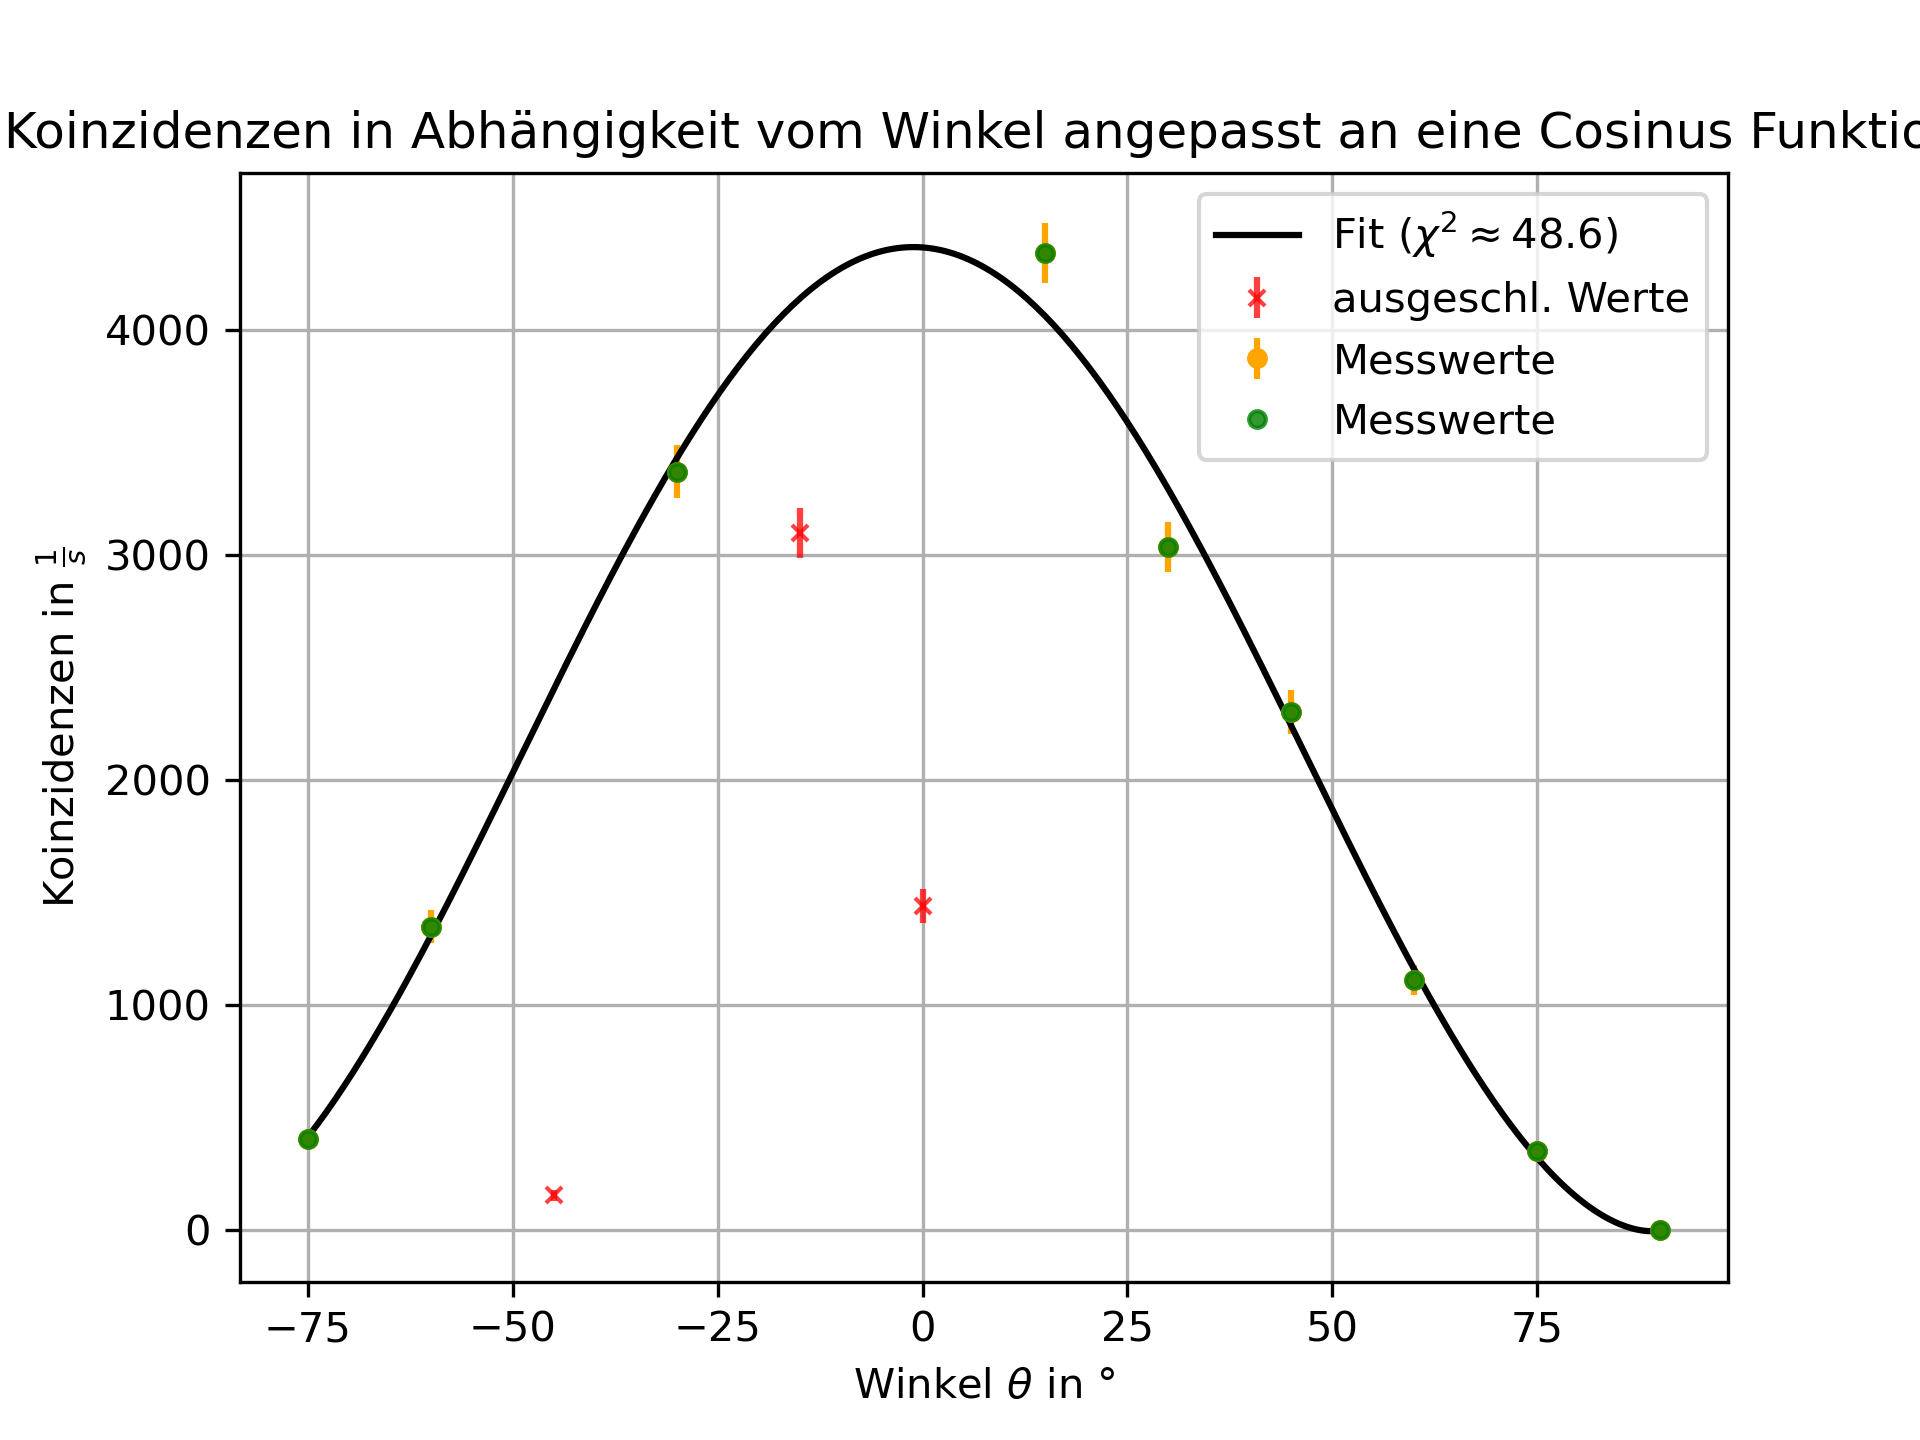
\includegraphics[width=1\textwidth]{figures/cosAnpassung.png}
    \caption{Cosinus-Anpassung an die Winkelverteilung}
    \label{fig:WinkelverteilungCosinus}
\end{figure}

\begin{figure}[H]
    \centering
    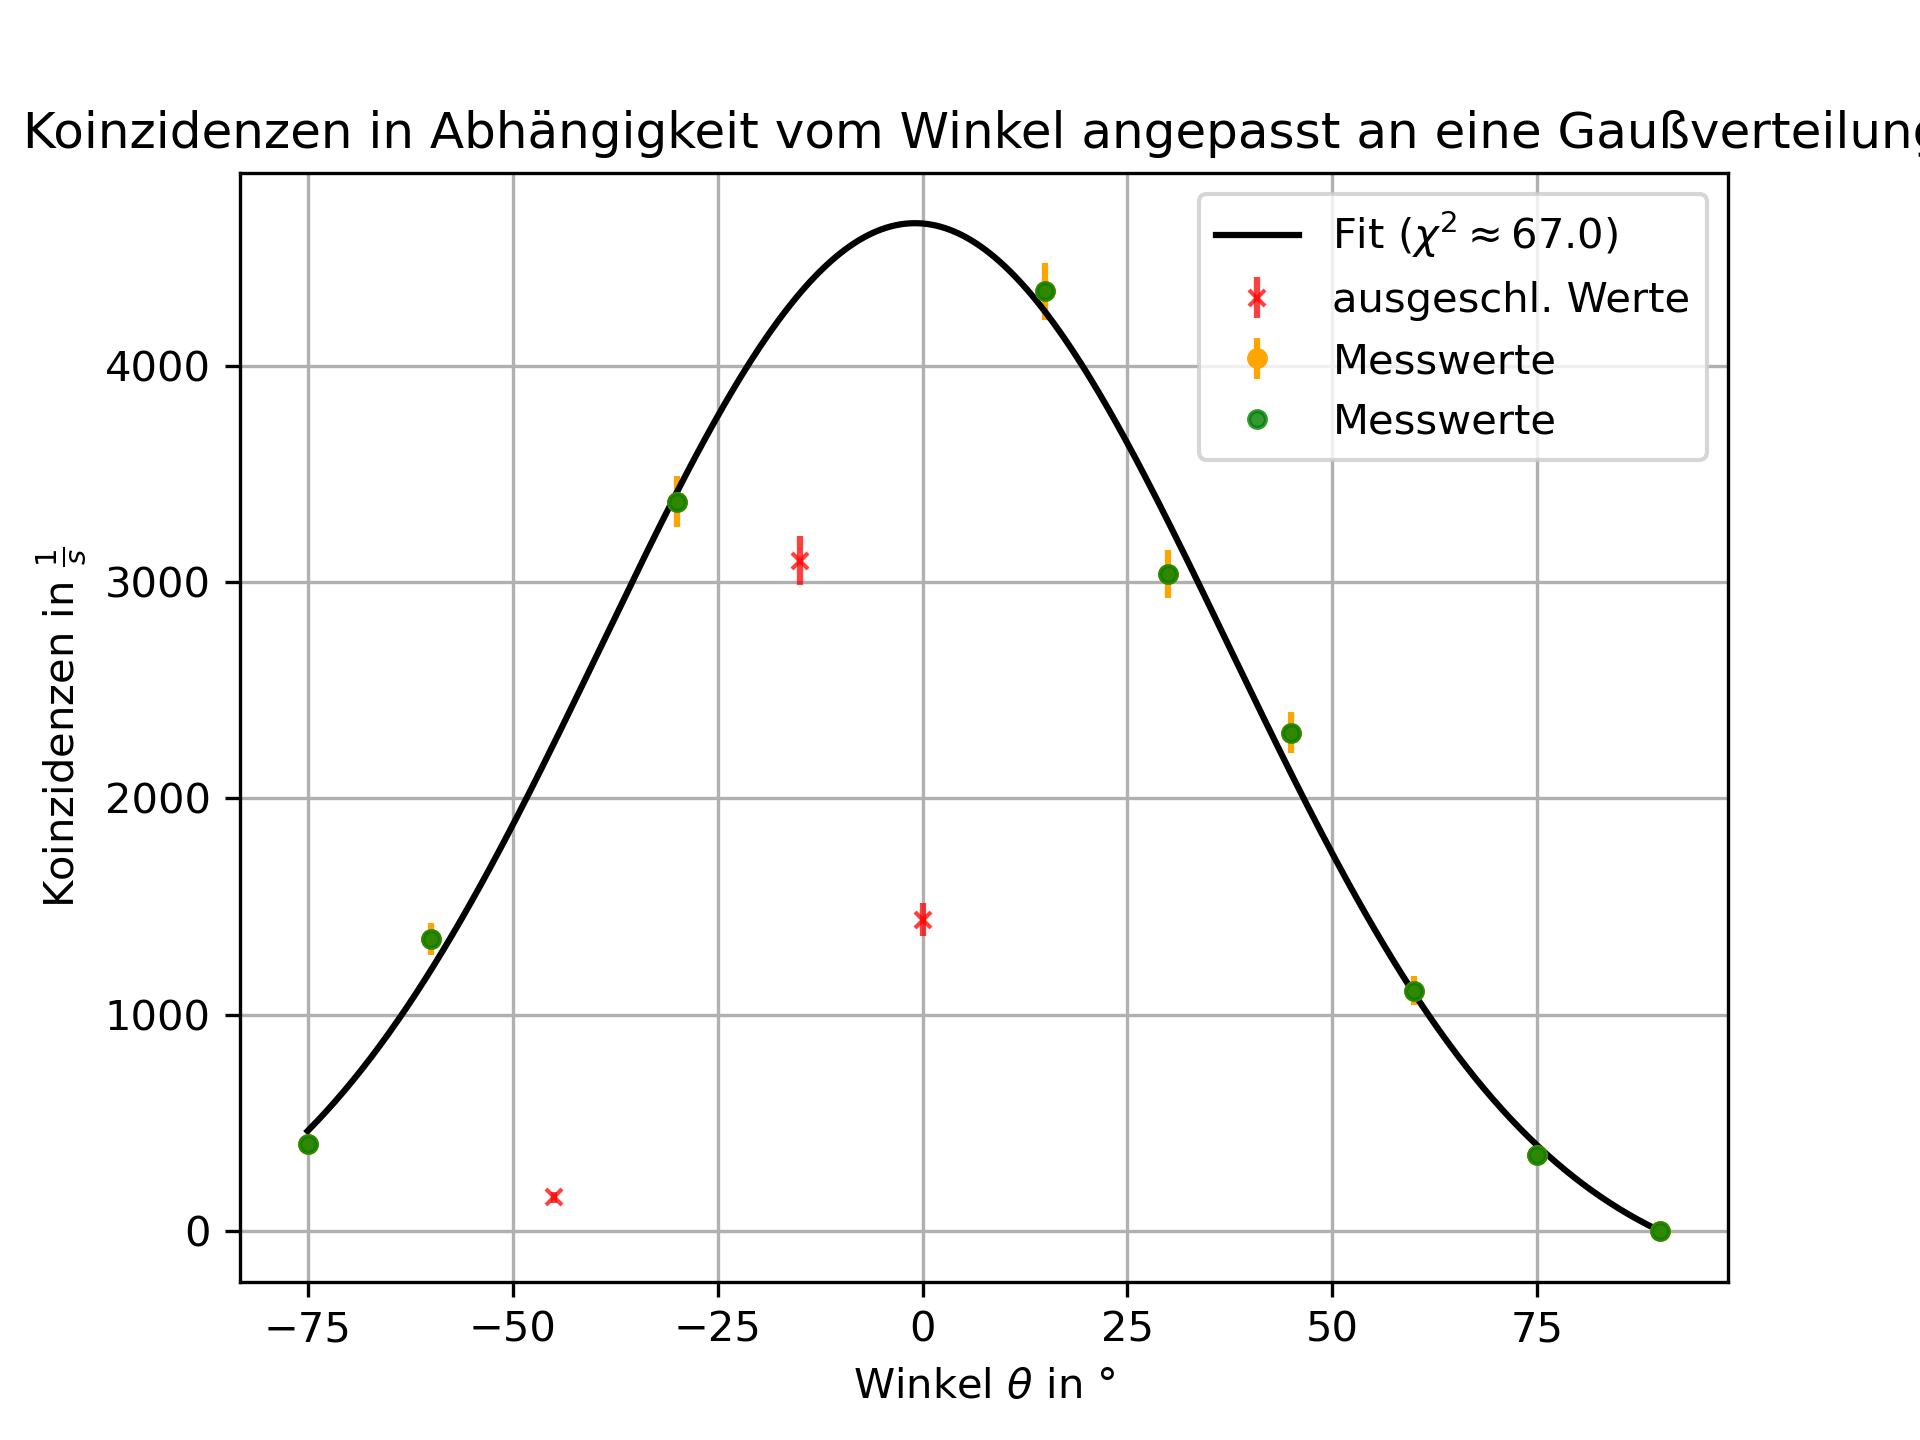
\includegraphics[width=1\textwidth]{figures/gaussAnpassung.png}
    \caption{Gauss-Anpassung an die Winkelverteilung}
    \label{fig:WinkelverteilungGauss}
\end{figure} 
Die Parameter der Cosinus-Anpassung sind in der Tabelle \ref{tab:CosinusAnpassungWinkelverteilung} und die der Gauss-Anpassung in der Tabelle \ref{tab:GaussAnpassungWinkelverteilung} zu finden.
\begin{table}[H]
    \centering
    \caption{Cosinus-Anpassung an die Winkelverteilung}
    \begin{tabular}{|c|c|}
        \hline
        Parameter & Wert \\ \hline
        $A$ & 4378(50) \\ \hline
        $\phi$ / $\radian$ & 0,020(8) \\ \hline
        $n$ & 1.82(6) \\ \hline
        $c$ & -08(35) \\ \hline
        $d$ & 03(20) \\ \hline
    \end{tabular}
    \label{tab:CosinusAnpassungWinkelverteilung}
\end{table}
\begin{table}[H]
    \centering
    \caption{Gauss-Anpassung an die Winkelverteilung}
    \begin{tabular}{|c|c|}
        \hline
        Parameter & Wert \\ \hline
        $A$ & 4949(49) \\ \hline
        $\mu$ & -0,016(4) \\ \hline
        $\sigma$ & -0,667(6) \\ \hline
        $b$ & -291(16) \\ \hline
    \end{tabular}
    \label{tab:GaussAnpassungWinkelverteilung}
\end{table}
Wie zu erwarten war ist die Cosinus-Anpassung besser als die Gauss-Anpassung, da die Winkelverteilung eine Cosinus-Verteilung ist. Dies ist zu erkennen an den $\chi^2$ der Anpassungen.
Genauer wurde eine $\cos^2$ Abhängigkeit festgestellt, da die Cosinus-Anpassung eine $n=1,82(6)$-Abhängigkeit hat, die nahe bei 2 liegt.

\subsubsection*{Pulshöhenspektrum}
Die Messung des Pulshöhenspektrums wurde in der Abbildung \ref{fig:PulshoheWinkelverteilung} aufgetragen.
Hierbei ist keine Landau-Verteilung zu erkennen, was aber auffällt ist, dass der Rauschanteil am Anfang des Spektrums sehr hoch ist.
Dies fiel uns schon direkt nach der Messung auf, daher haben wir hier auch einen weiteren Datensatz von einer anderen Gruppe erhalten, die das gleiche Experiment durchgeführt hat.
Im Vergleich zu unserem Spektrum \ref{PulshoheWinkelverteilung} sieht man im Spektrum der anderen Gruppe \ref{fig:PulshoheWinkelverteilungAndereGruppe} eine Landau-Verteilung und der Rauschpeak
ist deutlich kleiner.
Wir gehen davon aus, dass unsere Schwellspannung zu niedrig eingestellt war, sodass auch ein starker Rauschanteil im Spektrum zu sehen ist. Daher ist auch die Landau-Verteilung \enquote{verwaschen} da der Rauschanteil auch
bei höheren Pulshöhen zu sehen ist und damit sich mit dem der Landau-Verteilung überlappt.
Dies kann auch der Grundsein, warum bei der Winkelverteilung einige Detektoren deutlich mehr Rauschanteilgemessen haben und damit die Außreißer in der Winkelverteilung entstanden sind.
Bei der weiteren Auswertung wurde der Datensatz der anderen Gruppe verwendet.
Das Pulshöhenspektrum ohne den Rauschanteil ist in der Abbildung \ref{fig:PulshoheWinkelverteilungLandauOhneFit} zu sehen.
\begin{figure}
    \centering
    \includegraphics[width=1\textwidth]{figures/Pulshöhenspektrum_Landau_ohne_fit.png}
    \caption{Pulshöhenspektrum gezoomt auf den Landauanteil}
    \label{fig:PulshoheWinkelverteilungLandauOhneFit}
\end{figure}
Hier wurde ein Bereich von $100$ bis $800$ betrachtet.
In der Abbildung \ref{fig:PulshoheWinkelverteilungLandau} ist das Pulshöhenspektrum mit der Landau- und Gauss-Anpassung zu sehen.
Die Angepassten Funktionen sind in der Gleichung \ref{eq:LandauAnpassung} und \ref{eq:GaussAnpassungPulshohe} zu finden.
\begin{displaymath}
    L(x) = A \cdot exp\left[ -\frac{1}{2} \left( \frac{x - \mu}{\sigma} \right) + exp\left( -\frac{x - \mu }{\sigma} \right) \right] 
\label{eq:LandauAnpassung}
\end{displaymath}
\begin{displaymath}
    G(x) = A \cdot e^{-\frac{(x - \mu)^2}{2\sigma^2}} + b
\label{eq:GaussAnpassungPulshohe}
\end{displaymath}
Die Parameter der Anpassungen sind in der Tabelle \ref{tab:LandauAnpassungPulshohe} und \ref{tab:GaussAnpassungPulshohe} zu finden.
\begin{table}[H]
    \centering
    \caption{Landau-Anpassung an das Pulshöhenspektrum}
    \begin{tabular}{|c|c|}
        \hline
        Parameter & Wert \\ \hline
        $\mu$ & 257,54(83) \\ \hline
        $\sigma$ & 38.78(52) \\ \hline
        $A$ & 62,6(11) \\ \hline
    \end{tabular}
    \label{tab:LandauAnpassungPulshohe}
\end{table}
\begin{table}[H]
    \centering
    \caption{Gauss-Anpassung an das Pulshöhenspektrum}
    \begin{tabular}{|c|c|}
        \hline
        Parameter & Wert \\ \hline
        $\mu$ & 260,47(83) \\ \hline
        $\sigma$ & 41,5(5) \\ \hline
        $A$ & 59(1) \\ \hline
    \end{tabular}
    \label{tab:LandauAnpassungPulshohe}
\end{table}

Durch die Anpassungen ist zu erkennen, dass die Landau-Anpassung besser ist als die Gauss-Anpassung, da die $\chi^2$-Werte der Anpassungen deutlich kleiner sind.
Dies deutet wie erwartet darauf hin, dass es sich um ein dünnes Szintillationsmaterial handelt, da die Landau-Verteilung für dünne Szintillatoren typisch ist.


\subsubsection*{Zufallskoinzidenz}
Wie im Abschnitt \enquote{Zufallskoinzidenz} beschrieben, wurde die Zufallskoinzidenzrate auf 2 Arten bestimmt.
Für die zeitliche Zufallskoinzidenzrate wurde eine Zeitverzögerung von $\SI{20}{\micro\second}$ für den Diskriminator $D25$, $\SI{90}{\micro\second}$ für den Diskriminator $D14$ und 
$\SI{165}{\micro\second}$ für den Diskriminator $D2$ gewählt, dabei kommen je $\SI{5}{\micro\second}$ durch die minimal Verzögerungszeit \cite{}.
Die räumliche Zufallskoinzidenz war die Verteilung der Detektoren vorausgewählt, diese waren in einem rechtwinkligen Dreieck angeordnet, sodass ein einzelnes Teilchen keine Koinzidenz erzeugen kann.
Damit die Zufallskoinzidenz bestimmt werden kann muss zunächst eine theoretische Zufallskoinzidenzrate bestimmt werden.
Die durchschnittliche Überlagerung für n-Signale der Szintillatoren ist gegeben mit:
\begin{displaymath}
    \frac{1}{\Delta t}= \sum_{i=1}^{n} \frac{1}{\t_i}
\end{displaymath}
Dabei ist $\Delta t$ die Zeit der überlagerten Signale, $n$ die Anzahl der Signale und $\Delta t_i$ die Zeit, in der das i-te Signal vorhanden ist.
Die Rate daraus erhalten wir durch:
\begin{displaymath}
    f=\Sigma_{i=1}^{n} (f_i \Delta t_i) \cdot \frac{1}{\Delta t_i}
\end{displaymath}
Die Gesamtzahl an Ereignissen $N$ ist gegeben durch:
\begin{displaymath}
    N = f \cdot T
\end{displaymath}
wobei $T=\SI{598215}{\second}$ die gesamt Zeitdauer der Messung ist.
Daraus folgt die theoretische Zufallskoinzidenzrate für 3 Signale:
\begin{displaymath}
    N_3=T\Sigma_{i=1}^{3} (f_i \Delta t_i) \cdot \frac{1}{\Delta t_i}
\end{displaymath}
Dabei gilt $N_{25}=f_1 \cdot T$ und es folgt:
\begin{displaymath}
    N_3 = \frac{N_{25}^3}{T^2} \cdot \Sigma_{i=1}^{3} \sum_{i=1}^{3}\frac{1}{\Delta t_i}
\end{displaymath}
Mit $N_{25}=2993503$ und $T=\SI{598215}{\second}$ ergibt sich für die zeitliche Zufallskoinzidenzrate:
\begin{displaymath}
    N_3 = 1,5 \cdot 10^6    
\end{displaymath}
Da bei der räumlichen Zufallskoinzidenzrate auch bei 2 Signale gleichzeitig anliegen können, ergibt sich für die räumliche Zufallskoinzidenzrate:
\begin{displaymath}
    N_2 = 2,28
\end{displaymath}
Auch hier sind die Effekte der niedrigen Schwellenspannung zu erkennen, da die Zufallskoinzidenzrate deutlich höher ist als die theoretische Zufallskoinzidenzrate.
Aber Qualitativ entspricht das unseren Erwartungen, dass die zeitliche Zufallskoinzidenz fast bei 0 ist und die räumliche im gegensatz zu Theorie eine viel höhere Rate hat, da hier auch die
Rauscheffekte mit einfließen und diese auch schon von 2 Signalen ausgelöst werden kann. 

\section{Anhang}

\subsection{LABView-Programm}
\begin{figure}
    \centering
    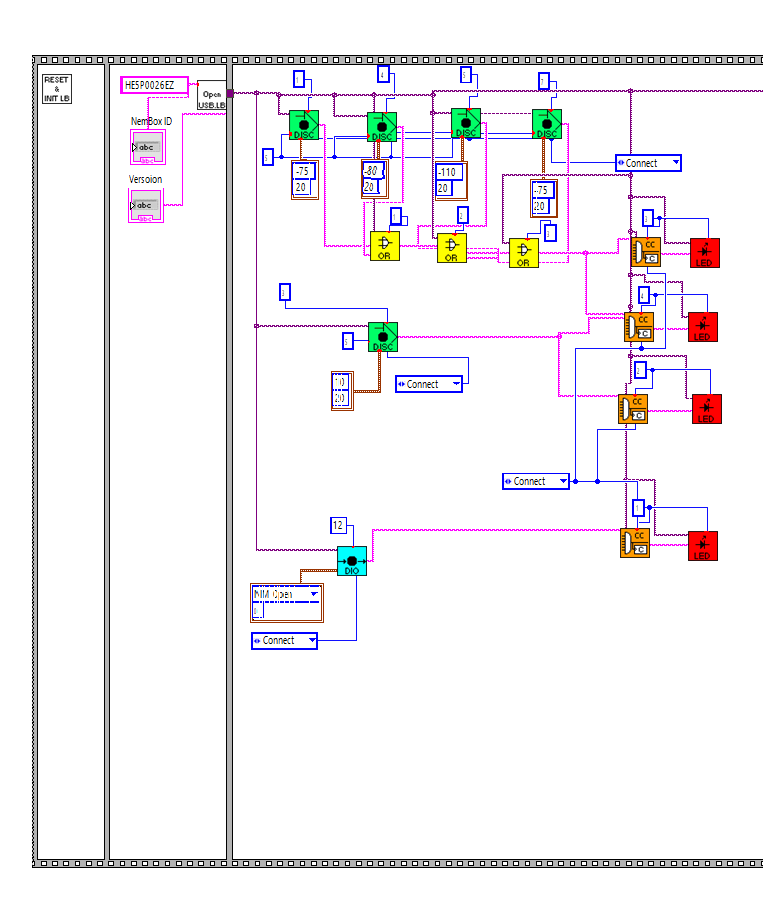
\includegraphics[width=1\textwidth]{figures/ProgrammScreen1.png}
    \caption{LABView-Programm zur Schwellenspannungseinstellung Teil 1}
    \label{fig:LABView1}
\end{figure}
\begin{figure}
    \centering
    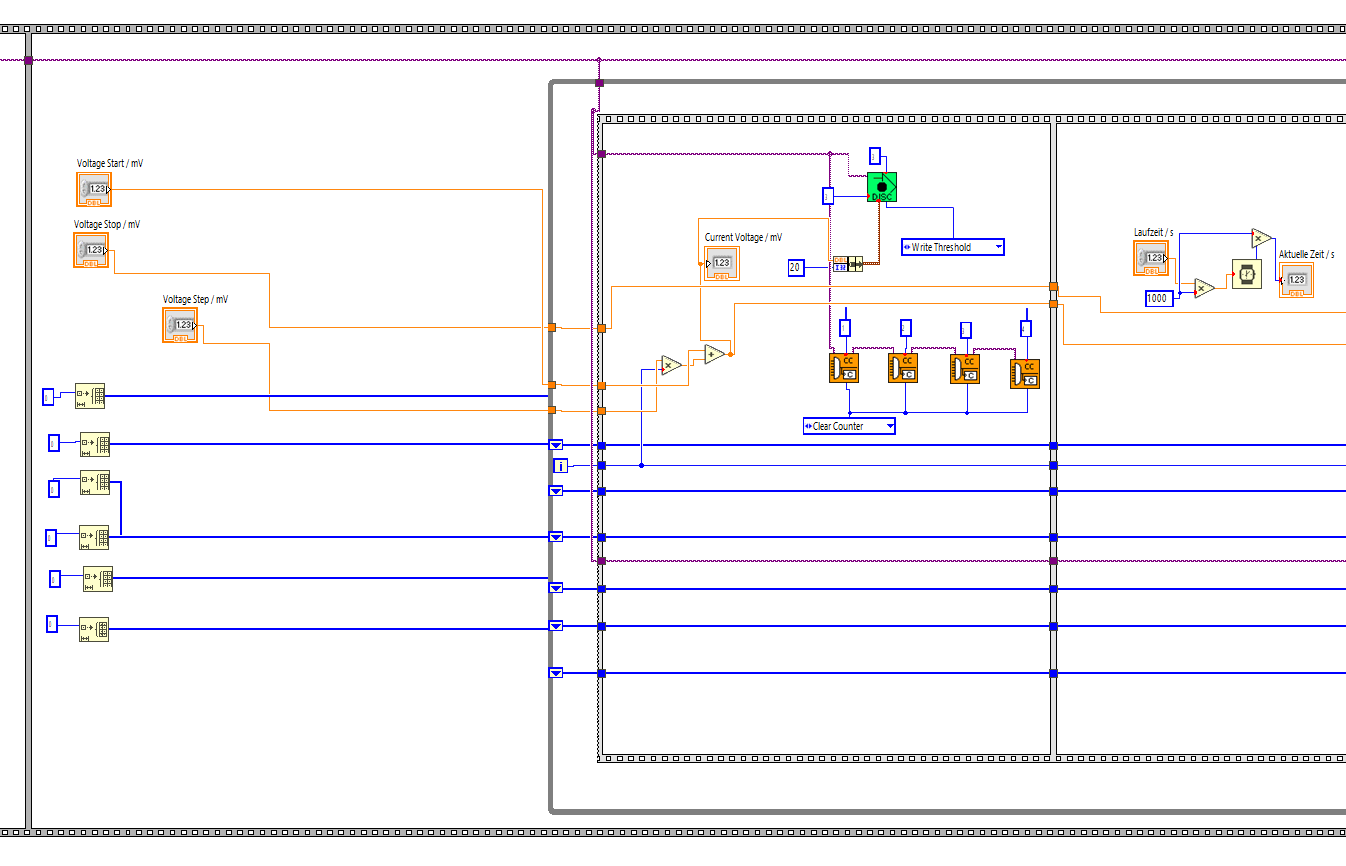
\includegraphics[width=1\textwidth]{figures/ProgrammScreen2.png}
    \caption{LABView-Programm zur Schwellenspannungseinstellung Teil 2}
    \label{fig:LABView2}
\end{figure}
\begin{figure}
    \centering
    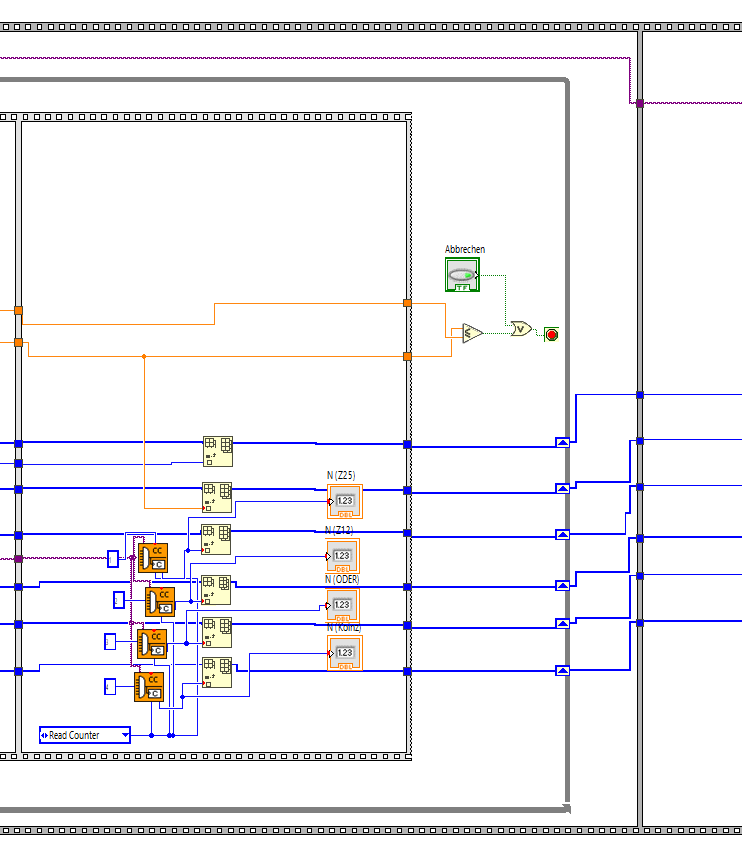
\includegraphics[width=1\textwidth]{figures/ProgrammScreen3.png}
    \caption{LABView-Programm zur Schwellenspannungseinstellung Teil 3}
    \label{fig:LABView3}
\end{figure}
\begin{figure}
    \centering
    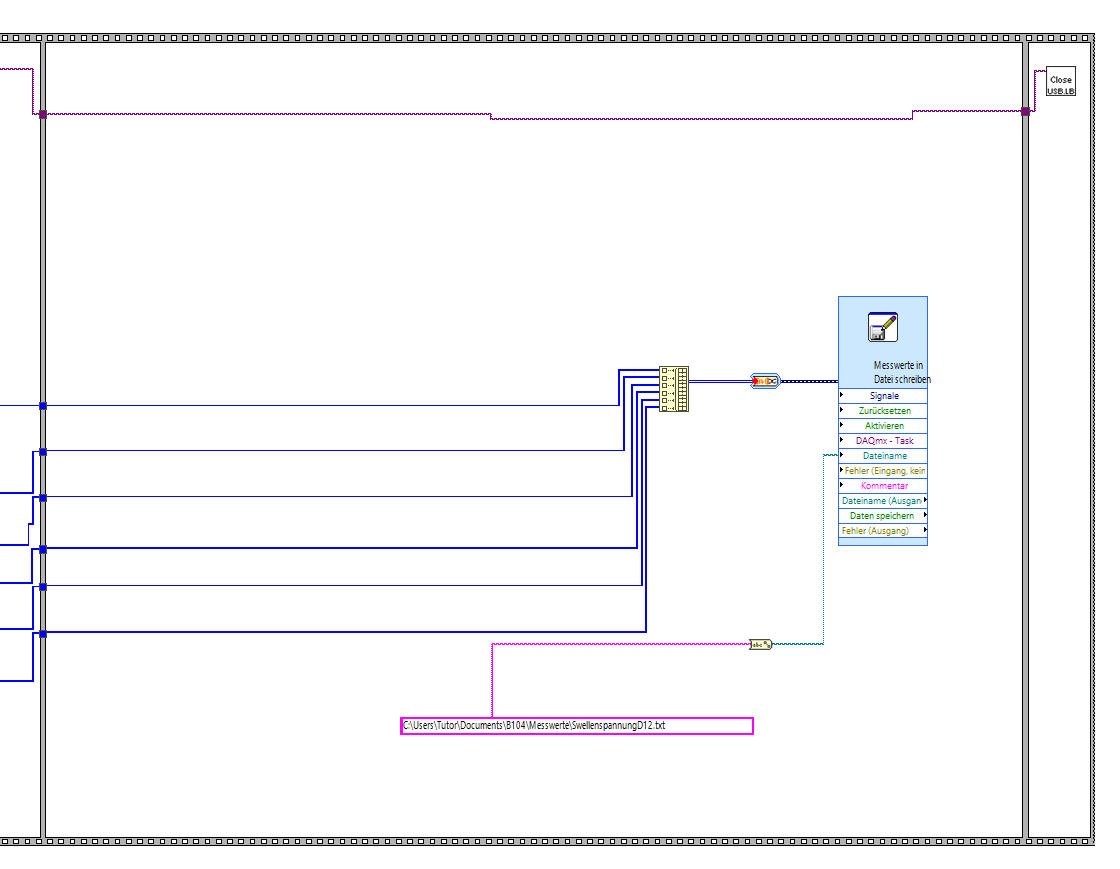
\includegraphics[width=1\textwidth]{figures/ProgrammScreen4.png}
    \caption{LABView-Programm zur Schwellenspannungseinstellung Teil 4}
    \label{fig:LABView4}
\end{figure}

\subsection*{Winkelverteilung}
\begin{table}[H]
    \centering
    \caption{Anpassungsparameter der Bestimmung der Schwellenspannung für die Winkelverteilung}
    \begin{tabular}{|c|c|c|}
        \hline
        $-U$ / mV & $N_\mathrm{Koin.}/N_{25}$ & $\Delta (N_\mathrm{Koin.}/N_{25})$ \\ \hline
        10 & 8.24e-03 & 6.89e-04 \\ \hline
        20 & 7.23e-03 & 6.39e-04 \\ \hline
        30 & 5.98e-03 & 5.83e-04 \\ \hline
        40 & 4.88e-03 & 5.27e-04 \\ \hline
        50 & 3.72e-03 & 4.56e-04 \\ \hline
        60 & 2.07e-03 & 3.40e-04 \\ \hline
        70 & 2.34e-03 & 3.61e-04 \\ \hline
        80 & 1.40e-03 & 2.81e-04 \\ \hline
        90 & 1.35e-03 & 2.75e-04 \\ \hline
        100 & 7.29e-04 & 2.02e-04 \\ \hline
        110 & 5.65e-04 & 1.79e-04 \\ \hline
        120 & 5.20e-04 & 1.73e-04 \\ \hline
        130 & 7.92e-04 & 2.12e-04 \\ \hline
        140 & 7.27e-04 & 2.02e-04 \\ \hline
        150 & 1.68e-04 & 9.71e-05 \\ \hline
    \end{tabular}   
    \label{tab:SchwellenspannungWinkelverteilung}
\end{table}

\begin{table}
    \centering
    \caption{Messwerte der Winkelverteilung}
    \begin{tabular}{|c|c|c|}
        \hline
        Winkel / $\degree$ & $N_\mathrm{Koin.}$ & $\Delta (N_\mathrm{Koin.})$ \\ \hline
        -1 & 405 & 20 \\ \hline
        -1 & 1349 & 37 \\ \hline
        -1 & 3372 & 58 \\ \hline
        0 & 4344 & 66 \\ \hline
        1 & 3037 & 55 \\ \hline
        1 & 2304 & 48 \\ \hline
        1 & 1111 & 33 \\ \hline
        1 & 351 & 19 \\ \hline
        2 & 0 & 0 \\ \hline
    \end{tabular}
    \label{tab:Winkelverteilung}
\end{table}

\begin{figure}
    \centering
    \includegraphics[width=1\textwidth]{figures/Pulshöhenspektrum_Unser.png}
    \caption{Pulshöhenspektrum der Winkelverteilungsmessung}
    \label{fig:PulshoheWinkelverteilung}
\end{figure}
\begin{figure}
    \centering
    \includegraphics[width=1\textwidth]{figures/Pulshöhenspektrum_B109.png}
    \caption{Pulshöhenspektrum der Winkelverteilungsmessung einer anderen Gruppe}
    \label{fig:PulshoheWinkelverteilungAndereGruppe}
\end{figure}
\newpage

\printbibliography[heading=bibintoc]

\end{document}